\begin{figure*}[p]
\centering

\newcommand{\codefile}[1]{%
    \lstinputlisting[
        style=mystyle,
        basicstyle=\fontsize{4.1}{4.5}\selectfont\ttfamily,
        frame=none,
        backgroundcolor=\color{white},
        aboveskip=1pt,
        belowskip=0pt,
        xleftmargin=1pt,
        xrightmargin=1pt
    ]{#1}%
}

\newcommand{\smalltitle}[1]{%
    {\fontsize{7}{7.5}\selectfont\bfseries #1}
}

\begin{tcolorbox}[
    width=\textwidth,
    colback=magenta!3,
    colframe=purple!40,
    title=Example with TikZ Code,
    enhanced,
    sharp corners=south,
    boxrule=0.5pt,
    left=2mm,
    right=2mm,
    top=1mm,
    bottom=1mm
]

\begin{minipage}[t]{0.29\linewidth}
\centering
\smalltitle{Source}

\vspace{1mm}

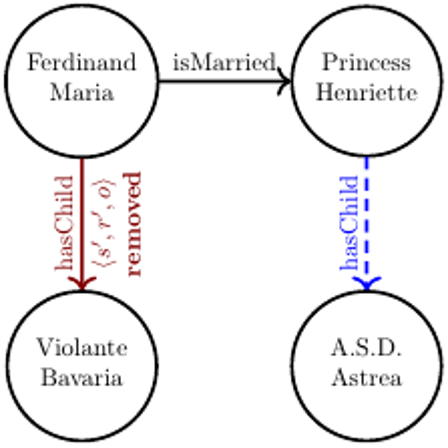
\includegraphics[
    width=\linewidth,
    height=2.9cm,
    keepaspectratio
]{structure/examples_new/sample_0066_source.png}
\end{minipage}
%
\hfill
%
\begin{minipage}[t]{0.36\linewidth}
\centering
\smalltitle{Edit Instruction}

\vspace{-2mm}

\begin{tcolorbox}[
    colback=white,
    colframe=gray!45,
    boxrule=0.3pt,
    arc=1mm,
    left=1mm,right=1mm,
    top=1mm,bottom=1mm
]
\raggedright
\fontsize{5.4}{6.1}\selectfont
The node labeled 'A.S.D. Astrea' and the blue dashed arrow connecting 'Princess Henriette' to it are removed from the diagram. The arrow connecting 'Ferdinand Maria' to 'Violante Bavaria' is changed from a solid red line to a solid black line. The text annotation '$\langle s',r',o\rangle$ removed' located below the arrow between 'Ferdinand Maria' and 'Violante Bavaria' is removed. A new blue dashed arrow labeled 'hasChild' is added, connecting 'Princess Henriette' to 'Violante Bavaria'. A text block reading 'target prediction $\langle s,r,o\rangle$' is added to the bottom right, with an arrow pointing from it to the new blue dashed arrow.
\end{tcolorbox}
\end{minipage}
%
\hfill
%
\begin{minipage}[t]{0.29\linewidth}
\centering
\smalltitle{Ground Truth}

\vspace{1mm}

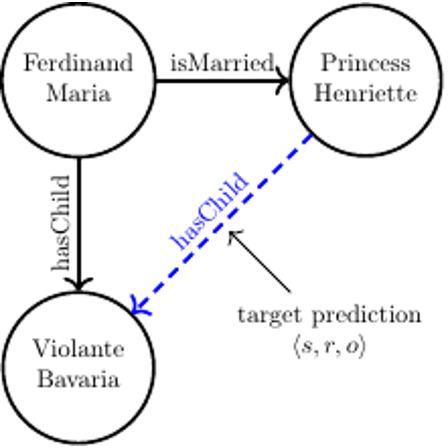
\includegraphics[
    width=\linewidth,
    height=2.9cm,
    keepaspectratio
]{structure/examples_new/sample_0066_gt.png}
\end{minipage}

\vspace{2mm}

\begin{minipage}[t]{0.44\linewidth}
\vspace{0pt}
\begin{tcolorbox}[
    width=\linewidth,
    colback=white,
    colframe=gray!45,
    boxrule=0.3pt,
    arc=1mm,
    left=0.5mm,right=0.5mm,
    top=0.5mm,bottom=0.5mm
]
\codefile{structure/examples_new/sample_0066_source.tex}
\end{tcolorbox}
\end{minipage}
%
\hfill
%
\begin{minipage}[t]{0.44\linewidth}
\vspace{0pt}
\begin{tcolorbox}[
    width=\linewidth,
    colback=white,
    colframe=gray!45,
    boxrule=0.3pt,
    arc=1mm,
    left=0.5mm,right=0.5mm,
    top=0.5mm,bottom=0.5mm
]
\codefile{structure/examples_new/sample_0066_gt.tex}
\end{tcolorbox}
\end{minipage}

\vspace{1mm}

\tcblower

\begin{minipage}[t]{0.485\linewidth}
\centering
\smalltitle{GPT-5.6-Sol}

\vspace{1mm}

\begin{tikzpicture}
\node[inner sep=0] (img) {%
    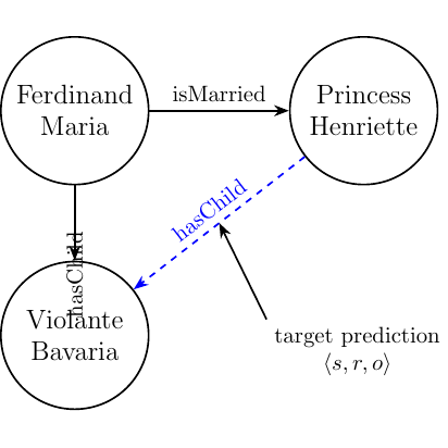
\includegraphics[
        width=0.72\linewidth,
        height=2.9cm,
        keepaspectratio
    ]{structure/examples_new/sample_0066_gpt.png}%
};

\node[
    anchor=west,
    right=1.5mm of img.east,
    align=left,
    fill=white,
    draw=gray!45,
    line width=0.3pt,
    rounded corners=1mm,
    inner xsep=1mm,
    inner ysep=0.8mm
] {%
    \fontsize{5.0}{5.8}\selectfont
    \begin{tabular}{@{}lr@{}}
    \textbf{TED}  & 0.716 \\
    \textbf{DSim} & 0.922 \\
    \textbf{EA}   & 1.000 \\
    \textbf{SP}   & 1.000 \\
    \textbf{VQ}   & 0.800 \\
    \textbf{AT}   & 334
    \end{tabular}
};
\end{tikzpicture}

\vspace{1mm}

\begin{tcolorbox}[
    colback=white,
    colframe=gray!45,
    boxrule=0.3pt,
    arc=1mm,
    left=0.5mm,right=0.5mm,
    top=0.5mm,bottom=0.5mm
]
\codefile{structure/examples_new/sample_0066_gpt.tex}
\end{tcolorbox}
\end{minipage}
%
\hfill
%
\begin{minipage}[t]{0.485\linewidth}
\centering
\smalltitle{EdiTikZ-9B-RL}

\vspace{1mm}

\begin{tikzpicture}
\node[inner sep=0] (img) {%
    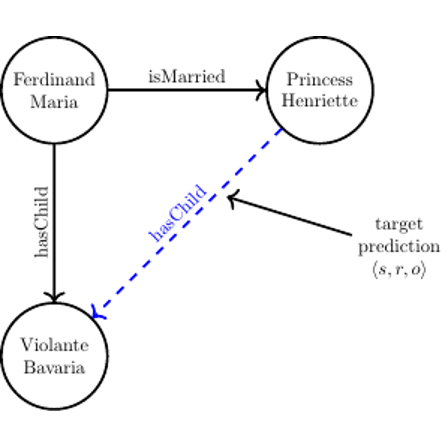
\includegraphics[
        width=\linewidth,
        height=2.9cm,
        keepaspectratio
    ]{structure/examples_new/sample_0066_9b_rl.png}%
};

\node[
    anchor=west,
    right=1.5mm of img.east,
    align=left,
    fill=white,
    draw=gray!45,
    line width=0.3pt,
    rounded corners=1mm,
    inner xsep=1mm,
    inner ysep=0.8mm
] {%
    \fontsize{5.0}{5.8}\selectfont
    \begin{tabular}{@{}lr@{}}
    \textbf{TED}  & 0.690 \\
    \textbf{DSim} & 0.918 \\
    \textbf{EA}   & 1.000 \\
    \textbf{SP}   & 1.000 \\
    \textbf{VQ}   & 1.000 \\
    \textbf{AT}   & 335
    \end{tabular}
};
\end{tikzpicture}

\vspace{1mm}

\begin{tcolorbox}[
    colback=white,
    colframe=gray!45,
    boxrule=0.3pt,
    arc=1mm,
    left=0.5mm,right=0.5mm,
    top=0.5mm,bottom=0.5mm
]
\codefile{structure/examples_new/sample_0066_9b_rl.tex}
\end{tcolorbox}
\end{minipage}

\end{tcolorbox}

\caption{TikZ programs and rendered figures for a representative scientific-figure edit. Models receive the source figure and edit instruction and generate the edited TikZ program. Per-example TED, DSim, EA, SP, VQ, and AT are shown beside each prediction.}
\label{fig:tikz_code_example}

\end{figure*}